
\section{\CRATE : Un éditeur décentralisé dans les navigateurs}
\label{editor:sec:crate}

\CRATE est un éditeur décentralisé permettant l'édition en temps réel de
documents dans les navigateurs Web. Cette section décrit son architecture avant
de détailler chacun des composants constituant cette architecture.

\begin{figure}
  \begin{center}
    \begin{tikzpicture}[scale=1.3]

\newcommand\X{25pt}
\newcommand\Y{20pt}

\newcommand\LIGHTGRAY{gray!20}
\newcommand\MEDIUMGRAY{gray!40}

\small
%% communication
\draw[rounded corners=2mm, color=\MEDIUMGRAY, fill=white](0pt, 0pt)+(-4*\X,-\Y)rectangle+(4*\X,\Y);
\draw(4*\X, \Y)node[anchor=north east]{\textbf{communication}};

\draw[fill=white](-2*\X, -0.25*\Y)
node{broadcast}+(-0.75*\X,-0.5*\Y)rectangle+(0.75*\X,0.5*\Y);
\draw[fill=white, very thick]( 0*\X, 0.25*\Y)
node[align=center]{membership}+(-0.85*\X,-0.5*\Y)rectangle+(0.85*\X,0.5*\Y);
\draw[fill=white]( 2*\X, -0.25*\Y)
node{unicast}+(-0.75*\X,-0.5*\Y)rectangle+(0.75*\X,0.5*\Y);

\draw[<-](-0.85*\X, 0.25*\Y)--(-1.25*\X, -0.25*\Y);
\draw[<-](0.85*\X, 0.25*\Y)--(1.25*\X, -0.25*\Y);

%% causality
\draw[rounded corners=2mm, color=\MEDIUMGRAY, fill=\LIGHTGRAY](0pt, -2*\Y)+(-4*\X,-\Y)rectangle+(4*\X,\Y);
\draw(4*\X, -\Y)node[anchor=north east]{\textbf{causality}};

\draw[fill=\LIGHTGRAY](-2*\X, -2*\Y)
node[align=center]{semantic\\[-1mm]causality\\[-1mm]tracker}
+(-1.0*\X,-0.6*\Y)rectangle+(1.0*\X,0.6*\Y);
\scriptsize
\draw[->, thick](-1.5*\X, -0.75*\Y) -- node[anchor=west]{receive}
(-1.5*\X, -1.4*\Y);
\draw[<-, thick](-2.5*\X, -0.75*\Y) -- node[anchor=east]{send}
(-2.5*\X, -1.4*\Y);
\small
\draw[<->]( 2*\X, -0.75*\Y)--( 1*\X, -2.5*\Y);

%% sequence structure
\draw[rounded corners=2mm, color=\MEDIUMGRAY, fill=white](0pt, -4*\Y)+(-4*\X,-\Y)rectangle+(4*\X,\Y);
\draw(4*\X, -3*\Y)node[anchor=north east, align=right]
{\textbf{sequence}\\\textbf{structure}};

\draw[fill=white, shading=axis,top color=\LIGHTGRAY, bottom color=white, shading angle=0](1*\X, -3*\Y)
node{anti-entropy}+(-0.95*\X,-0.5*\Y) rectangle +(0.95 *\X, 0.5*\Y);
\draw[fill=white, very thick](-2*\X, -4*\Y)
node{replica}+(-0.75*\X,-0.5*\Y) rectangle +(0.75 *\X, 0.5*\Y);

\draw[->] (0.05*\X, -2.75*\Y)--(-1*\X,-2*\Y);
\draw[->] (0.05*\X, -3.25*\Y)--(-1.25*\X,-4*\Y);
\scriptsize
\draw[<-, thick] (-1.5*\X, -3.5*\Y)--node[anchor=west]{deliver}(-1.5*\X, -2.6*\Y);
\draw[->, thick] (-2.5*\X, -3.5*\Y)--node[anchor=east]{decorate}(-2.5*\X, -2.6*\Y);
\small
%% gui
\draw[rounded corners=2mm, color=\MEDIUMGRAY, fill=\LIGHTGRAY](0pt, -6*\Y)+(-4*\X,-\Y)rectangle+(4*\X,\Y);
\draw(4*\X, -5*\Y)node[anchor=north east, align=right]
{\textbf{graphical}\\\textbf{user}\\\textbf{interface}};
\draw[fill=\LIGHTGRAY](0pt,-6*\Y)
node{web editor}+(-0.85*\X,-0.5*\Y) rectangle +(0.85 *\X, 0.5*\Y);

%%\draw[<->] (-2*\X, -4.5*\Y) -- (0*\X, -5.5*\Y);
\scriptsize
\draw[->, thick] (-1.80*\X, -4.5*\Y)--node[anchor=west]{notify}(-0.85*\X, -5.75*\Y);
\draw[<-, thick] (-2.20*\X, -4.5*\Y)--node[anchor=east]{update}(-0.85*\X, -6.25*\Y);
\small
\end{tikzpicture}
    \caption[Architecture de \CRATE]
    {\label{editor:fig:architecture}Architecture en 4 couches de \CRATE.}
  \end{center}
\end{figure}

La figure~\ref{editor:fig:architecture} montre l'architecture en 4 couches de
\CRATE. Chacune de ces couches peut devenir un obstacle au passage à l'échelle
de l'éditeur :
\begin{enumerate}[(i)]
\item la couche de communication comprend le mécanisme d'appartenance au réseau
  et la propagation des messages dans ce réseau;
\item la couche de causalité comprend la structure permettant de lier les
  opérations entre elles afin qu'elles soient intégrées dans un ordre reflétant
  une forme de causalité, e.g., elle assure que les opérations de suppression
  suivent toujours les opérations d'insertion de l'élément correspondant;
\item la couche de structure pour séquences dont les opérations d'insertions et
  de suppression doivent garantir des répliques convergeantes du document;
\item la couche d'interaction homme-machine fournissant les outils avec lesquels
  l'utilisateur peut interagir.
\end{enumerate}

\noindent La partie gauche de la figure montre le processus le plus courant :
Lorsqu'un participant effectue une opération sur le document, l'opération est
appliquée à la séquence répartie. L'opération est ensuite décorée avec des
métadonnées correspondant à la causalité. L'éditeur propage l'opération en
utilisant le voisinage de l'éditeur fournit par le protocole d'appartenance au
réseau.  À l'inverse, lorsque l'éditeur reçoit une opération, il vérifie si
cette dernière est prête à être intégrée. Lorsque la condition est vérifiée,
l'éditeur intègre l'opération à la réplique de la séquence. L'interface
utilisateur est notifiée du changement.

\noindent La partie droite de la figure correspond à la stratégie de rattrapage
où un participant a peut-être manqué quelques opérations à cause de pertes de
messages dans le réseau, ou simplement car il était hors-ligne pendant un
moment. Ainsi, dès que l'éditeur est en ligne, il vérifie régulièrement auprès
de ses voisins s'il lui manque des opérations~\cite{demers1987epidemic,
  vanderlinde2016delta}.


\subsection{Communications}

Les sessions d'édition peuvent rassembler de petits groupes comme de larges
groupes pendant leur durée de vie. Par exemple, un cours de formation en ligne
ouverte à tous (\emph{MOOC}) peut commencer avec un grand nombre d'étudiants
dont le nombre peut s'amoindrir très rapidement par de manque
d'intérêt~\cite{breslow2013studying}. De plus, les sessions d'édition varient en
taille selon la portée du document. Par exemple, un document décrivant un projet
personnel et dont la visibilité est limitée aux amis rassemble significativement
moins de monde qu'un document décrivant un grand événement, tel que le rapport
collaboratif d'une conférence. La couche de communication doit être en mesure de
gérer de manière transparente toute session d'édition, quelle que soit sa
taille, tout en passant à l'échelle.

\CRATE utilise \SPRAY (cf. chapitre~\ref{net:chap:spray}) afin d'ajuster
automatiquement son fonctionnement à la session d'édition. Ainsi, chaque éditeur
possède une vue partielle avec laquelle communiquer. La taille de cette dernière
croît et décroît logarithmiquement par rapport à la taille du réseau. Si une
session d'édition démarre avec 10 auteurs, ils auront 2.3 voisins en moyenne. Si
la session d'édition grandit pour atteindre le millier de participants, ceux-ci
auront 6.9 voisins en moyenne. Enfin, si l'édition se retrouve avec 10
participants à nouveau, ils auront à nouveau 2.3 voisins en moyenne.

La diffusion des messages fait un usage intensif des voisinages. Lorsqu'un
utilisateur procède à des changements dans le document, l'éditeur l'envoie à son
voisinage. Chacun des voisins ayant reçu le message le transmet à son tour à
son voisinages. Les modifications sur le document atteignent rapidement tous les
éditeurs par transitivité. La complexité en communication chez chaque éditeur
est bornée par $\mathcal{O}(M\ln(R))$, où $M$ est la taille du message, et
$R$ est le nombre de répliques connectées au moment de la propagation.

\begin{figure}
  \begin{center}
    
\begin{tikzpicture}[scale=1.3]

  \newcommand\X{30pt}
  \newcommand\Y{-30pt}
  
  \small

  \draw[->] (\X, 0)--(\X, 5+3*\Y); %% p1 p6
  \draw[->] (-5+2*\X, 0)--(5+\X, 0); %% p2 p1
  \draw[->] (2*\X, 0) -- (-5+3*\X, \Y); %% p2 p3
  \draw[->] (2*\X, 0) -- (-5+3*\X, 2*\Y); %% p2 p4
  \draw[->] (3*\X, 5+\Y) -- ( 5+2*\X, 0); %% p3 p2
  \draw[->] (3*\X, \Y) -- (5pt, 2*\Y); %% p3 p7
  \draw[->] (3*\X, \Y) -- (2*\X, 5+3*\Y); %% p3 p5
  \draw[->] (3*\X, 2*\Y) -- (5pt, 2*\Y); %% p4 p7
  \draw[->] (3*\X, 2*\Y) -- (5pt, \Y); %% p4 p8
  \draw[->] (2*\X, 3*\Y) -- (\X, -5pt); %% p5 p1
  \draw[->] (5+2*\X, 3*\Y) -- (3*\X, -5+ 2*\Y); %% p5 p4
  \draw[->] (-5+\X, 3*\Y) -- (0pt, -5+2*\Y); %% p6 p7
  \draw[->] (0pt, 2*\Y) -- (-5+3*\X, \Y); %% p7 p3
  \draw[->] (0pt, 2*\Y) -- (\X, -5pt); %% p7 p1
  \draw[->] (0pt, \Y) -- (2*\X, -5pt); %% p8 p2
  \draw[->] (0pt, \Y) -- (\X, 5+3*\Y); %% p8 p6
  \draw[->] (0pt, \Y) -- (-5+3*\X, \Y); %% p8 p3
  
  \draw[fill=white] (-2*\X, 1.5*\Y) node{$e_9$} +(-5pt,-5pt) rectangle +(5pt,5pt);
  \draw[<->, densely dashed, color=darkblue, very thick]
  (-2*\X, 5+1.5*\Y) -- node[anchor=east]{\DARKBLUE{join}} (-2*\X, -5pt);

  \draw[fill=white] (-2*\X, 0) node{$mediator_1$} +(-20pt, -5pt)rectangle+(20pt, 5pt);
  \draw[<->, densely dashed, color=darkblue, very thick]
  (20-2*\X, 0) -- node[anchor=south]{\DARKBLUE{share}} (-5+\X, 0);
  \draw[<->, densely dashed, color=darkblue, very thick]
  (20-2*\X, -5pt) -- (-5pt, \Y);
  
  \draw[fill=white] (-2*\X, 3*\Y) node{$mediator_2$} +(-20pt, -5pt)rectangle+(20pt, 5pt);
  \draw[<->, densely dashed, color=darkblue] (20-2*\X, 3*\Y) -- (-5+\X, 3*\Y);
  \draw[<->, densely dashed, color=darkblue] (20-2*\X, 5+3*\Y) -- (-5pt, 2*\Y);

  \draw[fill=white] (\X, 0)node{$e_1$}+(-5pt, -5pt)rectangle+(5pt, 5pt);
  \draw[fill=white] (2*\X, 0)node{$e_2$}+(-5pt, -5pt)rectangle+(5pt, 5pt);
  \draw[fill=white] (3*\X, \Y)node{$e_3$}+(-5pt, -5pt)rectangle+(5pt, 5pt);
  \draw[fill=white] (3*\X, 2*\Y)node{$e_4$}+(-5pt, -5pt)rectangle+(5pt, 5pt);
  \draw[fill=white] (2*\X, 3*\Y)node{$e_5$}+(-5pt, -5pt)rectangle+(5pt, 5pt);
  \draw[fill=white] (1*\X, 3*\Y)node{$e_6$}+(-5pt, -5pt)rectangle+(5pt, 5pt);
  \draw[fill=white] (0 , 2*\Y)node{$e_7$}+(-5pt, -5pt)rectangle+(5pt, 5pt);
%  \draw[fill=white] (0 , \Y)+(-55pt, -10pt)rectangle+(5pt, 10pt);
  \draw[fill=white](0,\Y) node{$e_8$}+(-5pt, -5pt)rectangle+(5pt, 5pt);

\end{tikzpicture}
    \caption[Fonctionnement d'une session d'édition]
    {\label{editor:fig:entering}Fonctionnement d'une session d'édition.}
  \end{center}
\end{figure}

La figure~\ref{editor:fig:entering} décrit le processus d'entrée dans le réseau.
Une session d'édition, composée de 8 éditeurs existe. Celle-ci est inaccessible
depuis l'extérieur. Pour rejoindre le réseau, au moins un des éditeurs doit
partager son accès. Pour ce faire, il crée une connexion avec un serveur de
signalisation facilement accessible via \emph{websocket}. L'éditeur ayant
partagé son accès donne à son collègue une adresse URL contenant suffisamment
d'informations pour qu'il retrouve le médiateur et demande à rejoindre la
session d'édition. Lorsqu'il clique sur l'adresse, une connexion est établie
avec le serveur de signalisation qui va jouer le rôle de médiateur afin de créer
le premier canal de communication WebRTC entre le nouveau membre et l'éditeur
partageant l'accès. Une fois celui-ci établi, le nouvel arrivant se déconnecte
du médiateur et applique le protocole \SPRAY en utilisant le canal
WebRTC. Ensuite, les éditeurs eux-mêmes deviennent des médiateurs et permettent
d'établir les connexions WebRTC d'un voisinage à l'autre.

\subsection{Détection de causalité}

Pour préserver des répliques cohérentes, le même résultat doit advenir lors de
la création de l'opération et de son intégration. Souvent, le comportement d'une
opération dépend d'autres opérations précédemment intégrées. Par exemple, la
génération d'une suppression nécessite l'existence de l'élément ciblé, et donc,
que l'opération d'insertion de cet élément soit intégrée. Ces relations de
précédence (\emph{happens before})~\cite{lamport1978time} contraignent l'ordre
d'intégration des opérations.  Malheureusement, l'ordre causal est très coûteux
: maintenir les relations causales d'une opération par rapport à toutes les
autres nécessite au minimum $\mathcal{O}(W)$ où $W$ est le nombre de
participants ayant effectués au moins une
opération~\cite{charronbost1991concerning}. La réception causale introduit dans
la complexité en communication un facteur linéaire sur le nombre de
participants. Si cela reste acceptable pour les petits groupes, le coût devient
trop élevé pour les grands groupes.

%la taille des messages confine l'utilisation de telles contraintes sur l'ordre
%d'intégration à de petites sessions d'édition bien contrôlées.

\CRATE ne contraint l'ordre d'intégration que pour les paires d'opérations liées
sémantiquement, c'est à dire que la suppression d'un élément suit toujours son
insertion. Si les opérations sont réceptionnées dans le désordre, la suppression
attend l'insertion correspondante. En revanche, les insertions sont
immédiatement intégrées lorsqu'elles sont reçues. Pour caractériser ces
relations causales, \CRATE utilise un vecteur d'horloges avec
exceptions~\cite{malkhi2007concise, mukund2014optimized}. Ce vecteur stocke pour
chaque participant
\begin{inparaenum}
\item un entier désignant le compteur maximal connu de ce participant et
\item une liste d'entiers désignant les exceptions, à savoir les opérations de
  ce participants dont l'existence est connue mais qui ne sont pas encore
  reçues.
\end{inparaenum}
Tandis qu'une telle structure conserve un surcoût local de l'ordre du vecteur
d'horloges $\mathcal{O}(W)$, le surcoût en communication devient constant
$\mathcal{O}(1)$.

\begin{figure}
  \begin{center}
    \begin{tikzpicture}[scale=1.3]
  
  \newcommand\X{ 20pt}
  \newcommand\Y{-30pt}

  \draw[->] (0pt,0pt) node[anchor=east]{$\pmb{c_1}$} -- (11*\X,0pt);
  \draw[->] (0pt,-30pt) node[anchor=east]{$\pmb{c_2}$} -- (11*\X,\Y);
  \draw[->] (0pt,-60pt) node[anchor=east]{$\pmb{c_3}$} -- (11*\X,2*\Y);

  \scriptsize
  \draw (0.5*\X,2+0*\Y) node[anchor=south]{[ ]} -- (0.5*\X,-2+0*\Y);
  \draw (0.5*\X,2+1*\Y) node[anchor=south]{[ ]} -- (0.5*\X,-2+1*\Y);
  \draw (0.5*\X,2+2*\Y) node[anchor=south]{[ ]} -- (0.5*\X,-2+2*\Y);

  \draw[->,densely dashdotted] (1.5*\X,0pt) -- (2.5*\X,2*\Y);
  \draw[->,densely dashdotted] (2.5*\X,0pt) -- (3.5*\X,1*\Y);
  \draw[->,densely dashdotted] (2.5*\X,0pt) -- (3.5*\X,2*\Y);


  \draw (5*\X,2+1*\Y) node[anchor=south]{[$\langle c_1,\,2,\,\DARKBLUE{\pmb{\{1\}}}\rangle$]}
  -- (5*\X,-2+1*\Y);
  \draw (5*\X,2+2*\Y) node[anchor=south]{[$\langle c_1,\,2,\,\varnothing\rangle$]}
  -- (5*\X,-2+2*\Y);

  \draw [->,densely dashdotted, very thick, color=darkblue]
  (1.5*\X,0pt) to[out=35,in=135] node[anchor=north]{\DARKBLUE{\textbf{slow}}}
  (6.65*\X,0pt) to[out=-45,in=110] (7.5*\X,\Y);

  \draw[fill=white] (1.5*\X,0pt) circle (2pt);
  \draw[fill=white] (2.5*\X,0pt) circle (2pt);

  \draw[->,densely dashdotted] (6*\X,2*\Y)--(6.5*\X,1*\Y);
  \draw[->,densely dashdotted] (6*\X,2*\Y)--(6.5*\X,0pt);

  \draw[fill=black] (6*\X,2*\Y) circle (2pt);
  
  \draw[->,densely dashdotted, very thick, color=darkblue]
  (6.5*\X,1*\Y)to[out=-35,in=-145]
  node[anchor=north]{\DARKBLUE{\textbf{wait}}}(8.5*\X,1*\Y);


  \draw (9.5*\X,2pt) node[anchor=south]
  {[$\langle c_1,\,2,\,\varnothing\rangle \langle c_3,\,1,\,\varnothing\rangle$]}
  -- (9.5*\X,-2pt);
  \draw (9.5*\X,2+1*\Y) node[anchor=south]
  {[$\langle c_1,\,2,\,\varnothing\rangle \langle c_3,\,1,\,\varnothing\rangle$]}
  -- (9.5*\X,-2+1*\Y);
  \draw (9.5*\X,2+2*\Y) node[anchor=south]
  {[$\langle c_1,\,2,\,\varnothing\rangle \langle c_3,\,1,\,\varnothing\rangle$]}
  -- (9.5*\X,-2+2*\Y);
  
  \begin{scope}[shift={(2*\X, 2.5*\Y)}]
  \draw[->,densely dashdotted] (0pt,-1pt) -- (10pt,-1pt)
  node[anchor=west]{messages};
  \draw[fill=white] (55pt,0pt)node[anchor=west]{$\,insert$}circle (2pt);
  \draw[fill=black] (92.5pt,0pt)
  node[anchor=west]{$\,delete(\langle c_1,\,1\rangle)$} circle (2pt);
  \end{scope}

\end{tikzpicture}

    \caption[Exemple de détection de relations causales]
    {\label{editor:fig:timeline}Exemple de détection de relations causales. Les
      triples dans les vecteurs sont composés de
      $\langle origin,\, max,\, exceptions\rangle$.}
  \end{center}
\end{figure}

La figure~\ref{editor:fig:timeline} montre une session d'édition impliquant 3
participants. Les vecteurs d'horloges avec exceptions sont initialisés vides. Le
collaborateur $c_1$ insère deux lettres dans le document et envoie les messages
correspondants. Le collaborateur $c_3$ reçoit rapidement les deux messages et
ajoute les identifiants des opérations à la structure de causalité. Les
opérations sont intégrées dans la séquence répliquée. Au même moment, le
collaborateur $c_2$ ne reçoit quant à lui que la seconde opération. Par
conséquent, il marque la première opération de $c_1$ en tant qu'exception et
intègre l'opération reçue. Le collaborateur $c_3$ supprime la première lettre
insérée par $c_1$ et en envoie le message. Tandis que $c_1$ intègre la
suppression immédiatement, $c_2$ doit attendre puisque l'opération d'insertions
ciblée appartient aux exceptions. Une fois l'opération manquante reçue,
l'exception disparaît et l'insertion est appliquée suivie de la suppression.

\subsection{Anti-entropie}

Lorsqu'un éditeur a besoin de récupérer l'état courant du document
(e.g. lorsqu'il rejoint la session d'édition), il exécute un mécanisme
d'anti-entropie.  Ce mécanisme a pour objectif de détecter les divergences entre
les répliques avant de les faire converger vers un état équivalent. À cela
s'ajoute la contrainte de ne perdre aucunes des modifications effectuées sur les
répliques. Le vecteur utilisé pour détecter les relations causales sert aussi
d'outil afin d'identifier les différences entre répliques. Le mécanisme
d'anti-entropie~\cite{demers1987epidemic, vanderlinde2016delta} fonctionne de la
façon suivante :
\begin{enumerate}[(i)]
\item Un éditeur choisit un éditeur de son voisinage aléatoirement et lui envoie
  son vecteur d'horloges avec exceptions.
\item L'éditeur recevant un tel vecteur effectue la différence, entrée par
  entrée, avec son propre vecteur. Ces différences permettent d'identifier les
  opérations manquantes qui sont alors envoyées en réponse.
\item L'éditeur recevant la réponse intègre les opérations normalement.
\end{enumerate}

\CRATE utilise donc une approche basée sur les opérations lorsqu'il fonctionne
normalement afin de permettre l'édition en temps réel. Lorsqu'il est en mode
hors ligne, ou si le réseau subit des perturbations, alors \CRATE utilise un
approche basée sur les différences. Le temps de convergence des répliques est
rapide grâce à la diffusion épidémique des messages, et fiable grâce au
mécanisme d'anti-entropie.


\subsection{Séquence répliquée}

La convergence forte à terme définit qu'un système est correct si les répliques
intégrant un même ensemble d'opérations convergent vers un état
équivalent~\cite{shapiro2011conflict}. La séquence répliquée a pour objectif de
garantir cette propriété de convergence des copies. Ainsi, les membres d'une
session d'édition lisent un document identique.

\CRATE utilise un type de données sans conflits conçu pour les
séquences afin de représenter ses documents. Un telle structure se base sur des
identifiants uniques et immuables. \CRATE utilise la fonction d'allocation \LSEQ
(cf. chapitre~\ref{repl:chap:lseq}) afin de fournir ces identifiants. Ainsi, les
suppressions suppriment réellement les éléments de la structure d'arbre
sous-jacente. De plus, la croissance de ces identifiants est bornée entre une
borne logarithmique et une borne polylogarithmique comparé au nombre
d'insertions dans la séquence. Étant sous-linéaire, la complexité en
communication devient acceptable. Étant sous-linéaire, la structure d'arbre
représentant le document répliqué n'a pas besoin d'être rééquilibré et donc,
l'éditeur n'a pas besoin d'exécuter un protocole de consensus qui ne passerait
pas à l'échelle~\cite{mostefaoui2015signature}.

Le facteur logarithmique de la dissémination de message, le coût constant
apporté par la détection de causalité, et le coût des identifiants implique une
complexité en communication attendue entre $\mathcal{O}((\log I)\cdot (\ln R))$ et
$\mathcal{O}((\log I)^2\cdot(\ln R))$ selon les comportements d'édition à l'œuvre,
où $I$ est le nombre d'insertions effectuées sur la séquence, et $R$ le nombre
de répliques dans la session d'édition au moment de la propagation de messages.


\subsection{Interface utilisateur}

Chaque participant possède une réplique du document partagé. Pourtant,
l'application doit donner l'illusion d'un unique document accédé par plusieurs
utilisateurs.

\CRATE est un éditeur temps réel -- écrit en HTML, CSS, et JavaScript -- qui
tourne directement dans les navigateurs Web. Il établit des canaux de
communication d'un navigateur à l'autre en utilisant la récente technologie
WebRTC~\cite{webrtc}. La zone de texte où l'utilisateur peut écrire est fournie
grâce à l'éditeur JavaScript Ace~\cite{ace}.

% Puisqu les CRDTs conçus pour les séquences fournissent des fonctions basées sur
% les identifiants plutôt que sur les indices, \CRATE doit utiliser une fonction
% \textsc{lookup} afin d'obtenir l'identifiant à l'indice voulu, et
% inversement. \TODO{Moar.}

% Les participants sont toujours en mesure de modifier le document lorsqu'ils le
% souhaitent.

\begin{figure}
  \begin{center}
    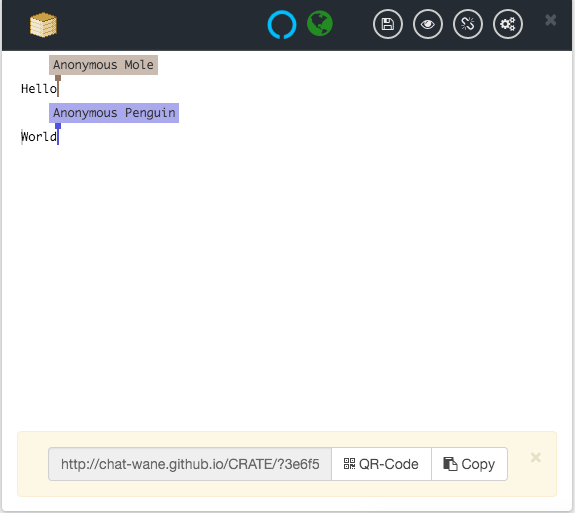
\includegraphics[scale=0.6]{img/editor/cratescreenshot.png}
    \caption[Capture d'écran de \CRATE]
    {\label{editor:img:screenshot}Capture d'écran de \CRATE.}
  \end{center}
\end{figure}

La capture d'écran en figure~\ref{editor:img:screenshot} montre l'interface
visible par l'utilisateur. Dans cet exemple, au moins trois participants sont
impliqués dans la session d'édition. En effet, 3 curseurs sont affichés. Le
premier curseur appartient à \emph{Anonymous Mole} et semble être à l'origine du
texte \emph{Hello}. Le second curseur appartient à \emph{Anonymous Penguin} et
semble être à l'origine du texte \emph{World}. Le troisième curseur est celui de
l'utilisateur ayant prit la capture d'écran.

La barre d'état nous indique que
\begin{inparaenum}[(i)]
\item l'éditeur est en train de partager l'accès à la session d'édition via le
  cercle bleue en rotation. L'utilisateur peut alors donner l'URL en bas de page
  à d'autres collaborateurs afin qu'ils le rejoignent dans l'écriture du
  document, en un simple clique;
\item que l'utilisateur est bien connecté à d'autres collaborateurs via la
  planète verte.
\end{inparaenum}

% La barre d'état possède aussi des boutons tels que
% \begin{inparaenum}[(i)]
% \item la disquette qui enregistre sur le disque la réplique locale du
%   document. En ouvrant ce fichier, l'éditeur est capable de se reconnecter à la
%   session d'édition sans avoir à rattraper toutes les opérations qui lui manque
%   depuis son départ;
% \item l'œil sert à visualiser le texte écrit dans le langage
%   Markdown~\cite{markdown}. Ainsi, le document n'est plus une simple suite de
%   caractères mais est interprété afin de présenter un document structuré plus
%   agréable à lire;
% \item la chaîne sert à partager l'accès au document ou à le stopper;
% \item les engrenages servent à la configuration.
% \end{inparaenum}

Le document lui-même peut contenir des URL référençant d'autres documents édités
en temps réel. D'un simple clique, un participant peut naviguer d'une session
d'édition temps réel à l'autre de manière décentralisée. Cette simple
fonctionnalité permet d'envisager la construction d'un Wikipédia à la fois
décentralisé et temps réel. 


%%% Local Variables:
%%% mode: latex
%%% TeX-master: "../../paper"
%%% End:
